\subsection{Spazio metrico}

\subsubsection{Distanza Euclidea}

\defn{Distanza Euclidea}{
Si definisce distanza euclidea tra \(\ux \) e \(\uy \) il numero reale non negativo definito da:

\[
    d(\ux,\uy) := \norm{\ux-\uy} = \sqrt{\prods{\ux-\uy}{\ux-\uy}} = \sqrt{\sum^n_{i=1} {(x_i - y_i)}^2}\ \ge 0
\]
\[
    d: \Rn \times \Rn \to \R^+_0
\]
}

La distanza euclidea verifica le proprietà della distanza:

\begin{enumerate}
    \item  \(d(\ux,\uy) \ge 0, \quad d(\ux,\uy) \in \R \)
    \item  \(d(\ux,\uy) = 0 \iff \ux =\uy \)
    \item  \(d(\ux,\uy) = d(\uy,\ux)\) \hfill (simmetria)
    \item  \(d(\ux,\uy) \le d(\ux,\underline{z}) + d(\underline{z},\uy),\ \ \forall \, \ux,\uy,\underline{z} \in \Rn  \) \hfill (disuguaglianza triangolare)
\end{enumerate}

\subsubsection{Definizione di spazio metrico}

\defn{Spazio metrico}{
    Si definisce spazio metrico un insieme della forma \(X, d\) con, \(X\) insieme, e \(d: X \times X \to \R^+_0\) un'applicazione che soddisfa le proprietà della distanza.

    Un esempio è il seguente:

    \[
        (\Rn ,d) \quad \text{con}\ d= \text{distanza euclidea}
    \]
}

Anche se noi useremo solo la distanza euclidea come metrica, esistono altri tipi di distanze con le quali è possibile definire rispettivi spazi metrici. Vediamone un paio:

\subsubsection*{Distanza Taxicab (o Manhattan)}

\[
    \ux=(x_1,x_2),\ \uy=(y_1,y_2) \quad \forall \ux,\uy \in \R^2
\]
\[
    d_1(\ux,\uy) = |y_1-x_1| + |y_2-x_2|
\]

\subsubsection*{Distanza di Chebyshev (o degli scacchi)}

\[
    \ux=(x_1,x_2),\ \uy=(y_1,y_2) \quad \forall \ux,\uy \in \R^2
\]
\[
    d_2(\ux,\uy) = \max \{ |y_1-x_1|,\ |y_2-x_2| \}
\]

\filbreak{}

\subsubsection{Successioni convergenti in \texorpdfstring{\(\Rn{}\)}{Rn}}

\defn{Successione}{
    Consideriamo la successione:
    \[
        {\{{\ux}_n\}}_{\N} \subset \Rn
    \]
    come un elenco ordinato di numeri i cui elementi sono elementi di \(\Rn \).
    \[
        {\ux}_n = (\ux_n^1, \ux_n^2,  \ldots , \ux_n^n)\ \in \Rn
    \]

    si dice che converge a \(\ux \in \Rn \) se:

    \[
        \lim_{n \to +\infty} d({\ux}_n,\ux) = 0
    \]

    cioè:
    \begin{align*}
        \forall \varepsilon >0,\ \exists \bar{N} \in \N
        \giventhat[\Big]
        d(\ux_n, \ux ) < \varepsilon ~\forall n \ge \bar{N}
    \end{align*}
}

Questo significa che:
\[
    d(\ux_n, \ux ) = \norm{\ux_n - \ux} = \sqrt{{(\ux_n^1-\ux^1)}^2 + \cdots + {(\ux_n^n-\ux^n)}^2}
\]
tende a 0 per \(n \to +\infty \iff \) tutti gli \((\ux_{n}^{i} - \ux^{i}) =0\).

\proposizione{}{ Sia \( \{\ux_n\} \subset \Rn \) una successione in \(\Rn \). Si ha:

    \begin{enumerate}
        \item (\textbf{Unicità}) \( \{\ux_n\} \) ha massimo un unico limite (se \( \{\ux_n\} \) ammette limite questo è unico)
        \item (\textbf{Limitatezza}) ogni successione convergente è limitata, ovvero:

              \[
                  \exists \ux_0 \in \Rn ,\ M \in \R
                  \giventhat[\Big]
                  d(\ux_n,\ux_0) \le M \quad \forall n \in \N
              \]

        \item (\textbf{Sottosuccessione}) Se \( \{\ux_n\} \to \ux \) in \(\Rn \) allora ogni sua sottosuccessione \( \{\ux_{n_k}\} \) di \( \{\ux_n\} \) converge allo stesso limite (\(\ux \))
    \end{enumerate}

}

\pagebreak{}

\subsubsection{Elementi di topologia in \texorpdfstring{\(\Rn \)}{Rn}}

Sia \(\ux_0 \in \Rn \) fissato e \(\R \ni r>0\)

Si ha la seguente definizione

\defn{}{Si definisce \textbf{palla aperta}, o \textbf{disco aperto}, o \textbf{intorno sferico di centro} \(\ux_0\) \textbf{e raggio} \(r\) l'insieme che si indica con:

    \[
        B(\ux_0,r) := \{ \ux \in \Rn \giventhat d(\ux,\ux_0)<r\} \subset \Rn
    \]
}

\subsubsection*{In n=1}

\(x_0 \in \R, \quad r > 0\)

\(B(x_{0},r) = x \in \left( x_0-r,\ x_0+r \right)\)

\subsubsection*{In n=2}

\begin{center}
    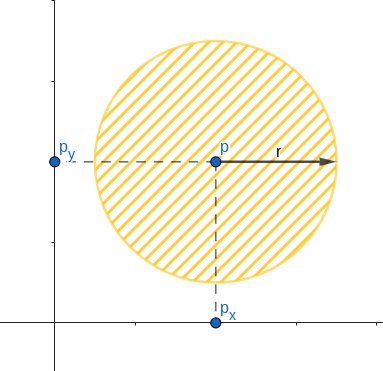
\includegraphics[scale=0.5]{intorno-sferico-r2.png}
\end{center}

\subsubsection*{In n=3}

\begin{center}
    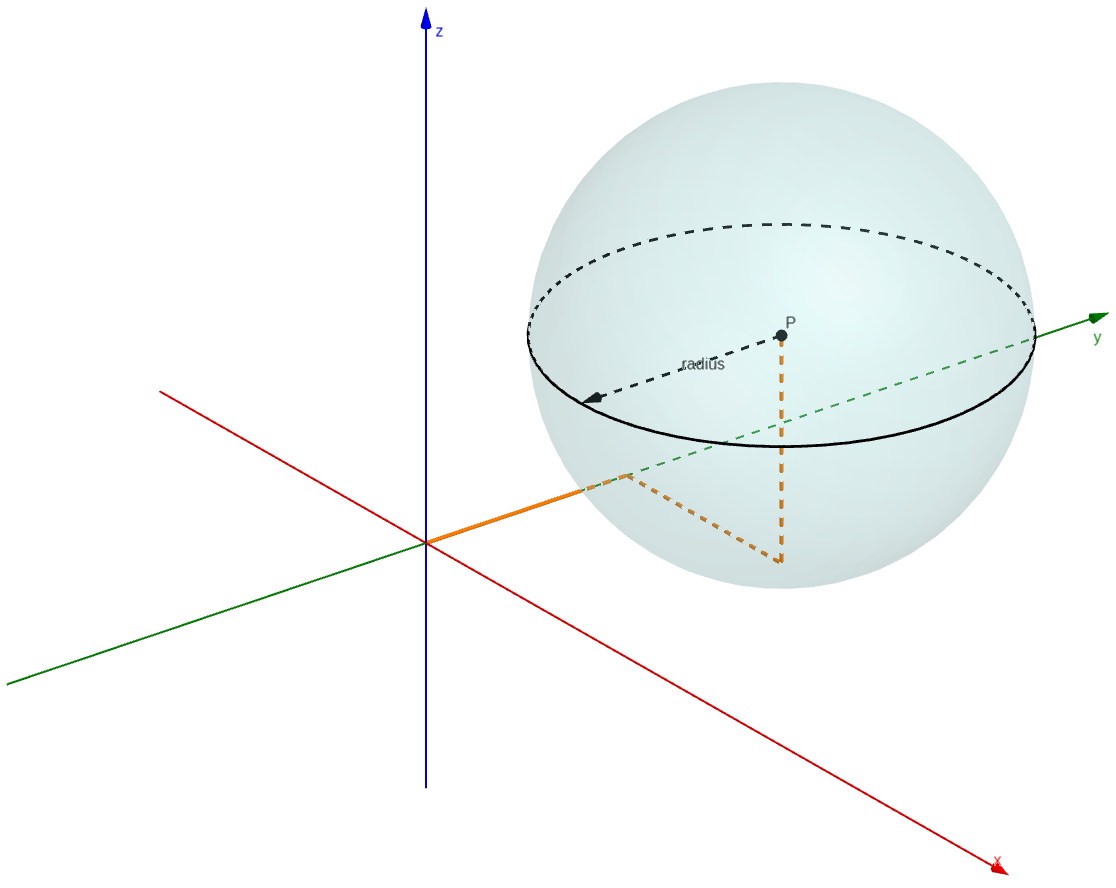
\includegraphics[width=\textwidth/2]{intorno-sferico-r3.png}
\end{center}

\filbreak{}

\subsubsection*{Esempio con distanza Euclidea e Taxicab}

\[
    (\R^{2},d) \rightarrow d(\ux,\uy) = \sqrt{\sum^{r}_{i=1} {(x_i-y_i)}^2}
\]

\[
    (\R^{2},d_1) \rightarrow d_1(\ux,\uy) = |x_1-y_1| + |x_2-y_2|
\]

se \(x_0=0\) e \(r=1\), questo è un cerchio:

\[
    B(\uzero,1) = \{\ux \in \R^2 \giventhat d(\ux,\uzero) <1\} = \{\ux \in \R^2 \giventhat \sqrt{{x_1}^2+{y_1}^2}<1\}
\]

e questo è un rombo (parallelogramma):

\[
    B(\uzero,1) = \{\ux \in \R^2 \giventhat d_1(\ux,\uzero) <1\} = \{\ux \in \R^2 \giventhat \underbrace{|x_1-0|}_{x_1} + \underbrace{|y_1-0|}_{y_1}<1\}
\]

\pagebreak

\subsubsection{Convergenza di successioni in uno spazio metrico}

Attraverso gli intorni sferici possiamo ridefinire il concetto di convergenza di successioni (limite) visto in precedenza.

\begin{align*}
    \{\ux_n\} \subset \Rn \text{ converge a } \ux_0 \in \Rn
    \iff
    \forall \varepsilon >0 ~\exists N_\varepsilon \in \N
    \giventhat[\Big]
    \ux_n \in B\left(\ux_0,\varepsilon\right) ~\forall n \ge N_\varepsilon
\end{align*}

\(
\ux_n \in B\left(\ux_0,\varepsilon\right) \implies \ux_n \text{ appartiene all'intorno sferico di centro } \ux_0 \text{ e raggio } \varepsilon
\)

\pagebreak

\subsubsection{Limitatezza in uno spazio metrico}

\defn{Insieme limitato}{
    \(A \subset X\) si dice \textbf{limitato} se esiste una palla aperta in cui \(A\) risulta interamente contenuto:

    \[
        \exists r>0,x_0 \in X \giventhat[\Big] A \subset B(x_0,r)
    \]

    e.g.{:} in \(X = \Rn \) con \(\ux_{0} = (0,0)\), \(A\) è limitato se è contenuto in un intorno sferico dell'origine, ovvero:

    \[
        \exists M > 0 \giventhat \norm{\ux} < M ~\forall \ux \in A
    \]
}

\defn{Punto interno}{
    Un punto di \(x_0 \in X\) si dice \textbf{interno} ad \(A\), con \(A \subset X\), se \(x_0 \in A\) e se esiste almeno un suo intorno sferico interamente contenuto in \(A\), ovvero:

    \[
        \exists r>0 \giventhat B(x_0,r) \subset A
    \]

    \(\mathring{A} =\) insieme dei punti interni di \(A\)
}

\defn{Punto esterno}{
    \(x_0 \in X\) si dice \textbf{esterno} ad \(A\) (\(A \subset X\)) se \(x_0 \notin A\) ed esiste almeno un suo intorno sferico completamente disgiunto da \(A\)

    \[
        \exists r>0 \giventhat[] B(x_0,r) \cap A = \emptyset
    \]
}

\defn{Punti di frontiera}{
    La frontiera di A si indica con il simbolo: \(\frontiera{A}\).

    I punti che non sono ne esterni, ne interni ad A, costituiscono la \textbf{frontiera} di A.
    Quindi, \(x_{0} \in \frontiera{A}\) se ogni suo intorno sferico contiene sia punti interni che punti esterni ad \(A\).
}

\defn{Punto di accumulazione}{

    Un punto \(\ux_0 \in A \subseteq \Rn \) si dice di \textbf{accumulazione} per \(A\) se ogni intorno sferico di \(\ux_0\) contiene almeno un punto di \(A\) diverso da \(\ux_0\), ovvero:

    \[
        \forall r > 0 \quad B(\ux_{0},r) \cap (A \setminus \{\ux_{0}\}) \neq \emptyset
    \]

    L'insieme dei punti di accumulazione di A si indica con il simbolo: \(D(A) = DA\)

    Esempi:
    \begin{itemize}
        \item I punti che costituiscono l'insieme dei punti interni di \(A = \mathring{A}\), sono punti di accumulazione
        \item I punti di frontiera, ovvero i punti di \(\frontiera{A}\) possono essere punti di accumulazione di \(A\) oppure no. Se il punto di frontiera non è di accumulazione, si chiama \textbf{punto isolato}.
    \end{itemize}
}

\defn{Chiusura di un insieme}{
    \textbf{Chiusura} di \(A \subset \Rn = \bar{A} = \mathring{A} \cup \frontiera{A} \qquad \) (interni + frontiera)

    Si può inoltre dimostrare che: \(\bar{A} = A \cup DA\)
}

\defn{Insieme aperto}{
    \(A \subset X\) si dice \textbf{aperto} se \(\mathring{A} = A\).

    E.g.: \(A \subset X\) è aperto se \(A = \emptyset \) oppure se ogni punto è un punto interno di \(A\).
}

\defn{Insieme chiuso}{
    Un insieme \(C \subset X\) si dice \textbf{chiuso} se contiene tutti i suoi punti di frontiera, ovvero, \(\frontiera{C} \subset C\)
}

\defn{Dominio}{
    Un dominio \(D\) in \(\Rn \) è la chiusura di un insieme aperto:

    \[
        D = \bar{A}  = A \cup \frontiera{A} \quad \text{con } A \text{ aperto}
    \]

    E.g.{:} in \(\Rn \) una sfera chiusa è un dominio: \( \{ \ux \in \Rn \giventhat \norm{\ux} \le M \} \) con \(M \in \N \) fissato.
}

\subsubsection*{Esempi di insiemi aperti}

\(A_1= \{ (x,y) \in \R^2 \giventhat x \neq y^2\} \)

\(A_2= \{ (x,y) \in \R^2 \giventhat x^2+ y^2 < 25\} \)

\(A_3= \{ (x,y) \in \R^2 \giventhat x^2+ 2y +1 \le 0\} \)
